\documentclass[]{article}

\usepackage{amsmath}
\usepackage[]{graphicx}
\usepackage{subfigure}
\usepackage[latin1]{inputenc}
\usepackage{comment}
\usepackage{url}
%\usepackage{biblatex} 
%\usepackage[pdftex]{graphicx}
\usepackage{color}
\usepackage{anysize}
\marginsize{3cm}{3cm}{2cm}{2.5cm}%l r t b

\title{Using an Open source face tracker for identity detection and facial expression Recognition}
%\title{Controlling a smart phone using gaze gestures}
%\title{Gaze gestures as an innovative HCI method for smartphone like devices}
 
\author{Eduardo Neiva, Jesus Nuevo, David Rozado}

\setlength\parindent{0pt} %no indentation in paragraphs
% Document starts
\begin{document}

\maketitle

\section{Abstract}
Face and eye tracking technology are fairly well developed and robust technologies. Eye tracking in combination with
gaze estimation permits the monitoring of the user's area of attention on a computer screen while also providing a hint
about possible intention. Facial tracking can augment eye tracking by monitoring facial features that can convey the
identity of the user or its internal cognitive state as expressed through its facial expression. In this work, we use an
open source face tracker that can recognize and classify facial expressions from continuous video input. The system uses
Constrained Local Models~\cite{saragih2011deformable} to this end. We
show that the face tracker is a powerful tool to recognize the
identity
of the user among a large pool of subjects. We also show that it can robustly recognize facial expressions of users on
which the system has been trained while also performing well on users
outside the training set. This positive
result and the open source nature of the system suggest the advantages of augmenting traditional eye trackers by
combining them with face tracking algorithms as the one suggested to enrich the set of features available to monitor a
human while interacting with a computer.


\section{Introduction}
Traditional Human Computer Interaction (HCI) could be augmented by providing computer systems with the ability to
recognize the emotions of the humans interfacing them. Emotions are conveyed by humans  using the visual, vocal
and other physiological means such as body gestures. Facial expressions are an indirect proxy to measure the internal
cognitive emotions of humans. Impaired facial expression recognition by humans can be a sign of serious cognitive
dysfunction such as schizophrenia \cite{Edwards2002789}.  Facial attributes can be tracked computationally through a
video stream of the subject's face. Making the computer aware of the emotions of the user could lead the way towards
more natural in fluid forms of interaction.


In this work we describe the usage of an open-source face tracker to feed a set of machine learning classifiers striving
to identify subjects identity and their facial expressions. The face
tracker provides a set of pose-invariant deformation parameters
estimated from the images. We use support vector machines (SVM)
to classify the invariant features provided by the face tracker.


The psychological literature has traditionally classified facial
expressions in six categories, in addition to the neutral expression:
anger, disgust, fear, joy, sadness and
surprise~\cite{schmidt2002human}. In this work, we also classify some additional facial gestures such as: raising
eyebrows, open mouth, kissing face, closed smile and squint face.


Researchers have employed a variety of methods to carry out facial expression recognition such as optical flow
computation  and symbolic representations \cite{Yacoob506414}, local binary patterns \cite{Shan2009803},  Bayesian
network classifiers \cite{Cohen1211408}, geometric deformation features and support vector machines
\cite{kotsia4032815}, hidden Markov models \cite{aleksic1597130, Cohen2003160}, Parametric flow models
\cite{blackAndYacoob}, AdaBoost and linear discriminant analysis \cite{bartlett1398364}. The surveys from
\cite{bartlett1398364} and \cite{Fasel2003259} are two good review sources about machine learning methods 
for fully automatic recognition of facial expressions. 


Previous work has employed a variety of techniques to classify  facial expressions. The work from \cite{Cohen2003160}
tested the classic neural network classifiers for classifying expression from video, focusing on changes in distribution
assumptions and feature dependency structures. The same authors also proposed and tested Hidden Markov Models (HMM) for
automatically segmenting and recognizing human facial expressions. Authors reported recognition rates up to 83\% for
frame-based recognition methods and 82\% for the multilevel HMM.


The work from \cite{Chen670976} investigated the emotional contents of speech and video based facial expression to
proposes a bioinspired algorithm for human facial expression recognition, concluding that both modalities can be
complimentary and able to achieve higher recognition rates than either modality alone. Authors in \cite{Busso:2004} also
used a multimodal approach to combine acoustic information and facial expression analysis in order to detect human
emotions. In their work, authors demonstrated that when both modalities are fused, the performance and the robustness of
the emotion recognition system improves considerably.


Bartlett et al.~\cite{Bartlett4624313} used perceptual primitives to code seven facial expressions in real-time. Their system
first detects frontal faces using a cascade of feature detectors trained with boosting techniques. The expression
recognizer receives image patches located by the phase detector. A Gabor representation of the parts is used  by a bank
of kernel based classifiers. Authors used a combination of Adaboost and support vector machines to enhance performance.
One of the most interesting properties of this work was its ability to change the outputs of the classifiers smoothly
as a function of time, hence, providing a dynamical representation of facial expression.

Databases available to the research community that include expression
labeling have appeared in last decade, of which the Cohn-Kanade
database~\cite{Cohn840611} is the best known. It contains over 2000
digitized image sequences from  182 adult subjects of varying
ethnicity, performing multiple tokens of most primary facial
expressions to create a comprehensive testbed for
comparative studies of facial expression analysis.


Facial identity recognition is another subject that has drawn a lot of attention in the research literature. While being
apparently trivial for humans to solve, automatic approaches have traditionally lagged behind the performance of humans
by at least one order of magnitude in terms of recognition performance. These approaches have only recently started to
catch up with the ability of the human brain to recognize faces \cite{onintelligence, Rozado2012b}. Face recognition is
important  for a wide range of commercial and law enforcement applications. Only recently has the technology required to
carry out automatic classification of faces become available. But the recognition of faces in outdoor environments 
where variation in pose and illumination are continuous remains a largely unsolved problem.

The work from \cite{Zhao:2003} provides a good literature survey on the subject of face recognition. In
\cite{Craw1987183}, authors undertake an in-depth discussion of face features automatic extraction for classification purposes of
grayscale images.

The work from \cite{Zhang20092876} undertakes a comprehensive review  of the challenging topic of pose invariant face
recognition, and while showing that the performance of different methods is still far from perfect, several promising
directions for future research  are suggested.

Authors in \cite{Tan20061725} review the also challenging topic of face recognition using  just one image per
class for training comparing several prominent algorithms for the tasks. the rationale for the study is the reported
critique that several face recognition techniques rely heavily on the size of the training set.

(i NEED TO COMPLETE THE LITERATURE REVIEW FOR IDENTITY RECOGNITION)

In summary, in this paper we apply that open source face tracker XXXXX for identity recognition and for facial
expression recognition. We suggest that facial tracking can be a powerful complement to traditional eye tracking  by
augmenting the set of features being tracked during human computer interaction. This  can potentially allow computer
systems to more precisely recognize the cognitive state of the human interfacing them through the proxy features of facial
dynamics.


\section{Methodology}

\subsection{Support Vector Machines}

Support vector machines (SVMs) have become popular as an efficient supervised learning model for classification. SVMs
work by generating a set of hyperplanes in a multiple dimensional space which is used for classification.  A good
classification is produced by maximizing the distances to the hyperplanes of the nearest training data points of the
different classes. Whenever the classification problem is not linearly separable in the hyperplane space, a technique
named kernel functions was introduced to map the original space into a much higher-dimensional space in order to achieve
linear separation.

Since SVMs make binary decision, a multi-class one-to-one classification was assigned for dealing with the several
classes (facial shapes) involved in our experiments. This work has used an open source SVM library called
LIBSVM\footnote{\url{http://www.csie.ntu.edu.tw/~cjlin/libsvm/}}. The library is available in many languages and
supports most of the functionality associated to SVM classification.

\subsection{Face Tracker}
The face tracker used in this work is the regularised landmark mean-shift of Saragih et
al.~\cite{saragih2011deformable}\footnote{Source code is available at
  \url{https://github.com/kylemcdonald/FaceTracker}} an extension of
the original Constrained Local Model (CLM) of Cootes et al.~\cite{cristinacce2006feature}. We only present these methods
here briefly, and refer the reader to the original articles. CLMs try to fit a trained model to an unseen face using a
set of local classifiers to detect points of interest independently, and using a global point distribution model (PDM),
also referred as the \textit{shape model} to constrain the relative position of the points. Figure~\ref{fig:CLM} illustrates the fitting process of CLM.

\begin{figure}[htbp]
  \centering
  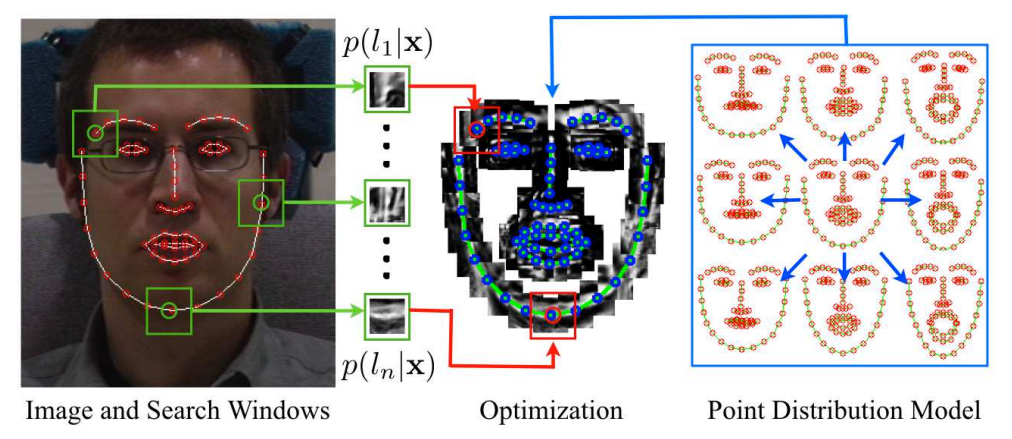
\includegraphics[width=12cm]{figures/CLM.png}
  \caption{Contrained Local Model fitting. The local patch classifiers generate surface responses, which are optimised
 together with the shape contraints. Courtesy of authors of~\cite{saragih2011deformable}.}
  \label{fig:CLM}
\end{figure}

The shape model is created from a training set. Non-rigid expressions are independent of the similarity transformation
of the face (scale, rotation and translation), so the shapes are transformed to a common reference frame and aligned,
typically using Procrustes method. From this set, the shape model is obtained using a dimensionality reduction technique
such as Principal Component Analysis (PCA). A new shape can then be generated as

\begin{equation}
  \label{eq:shape_model}
  \mathbf{x} = s\mathbf{R}(\bar{\mathbf{x}} +
  \boldsymbol{\Phi}\mathbf{q}) + \mathbf{t},
\end{equation}
were $\mathbf{x}$ is a vector with the landmark coordinates concatenated, 
$\{s,\mathbf{R},\mathbf{t}\}$ are the similarity transformation
parameters and $\mathbf{q}$ are the shape deformation parameters. The
shape model is defined by the \textit{mean shape} $\mathbf{\bar{x}}$
and the vectors of deformations $\boldsymbol{\Phi}$.

Patch classifiers are also created from a training
set. In~\cite{saragih2011deformable} the classifiers are linear SVMs,
which makes computation of the surface responses very fast. The
surface responses are composed with a sigmoid function, which output
can be treated as a probability map of the location of the
landmarks. These location of each landmark in it corresponding map is
then optimised with contrained mean-shift, where the locations are
updated using mean-shift independent of each other, and are then
constrained together by the shape model described above.



\subsection{Experimental Setup}
The dataset that was used to train and test the classification algorithms was specifically generated for this work. We
generated the data set from scratch instead of using existing data sets of facial expressions in order to gain freedom
in terms of the number of facial shapes available for testing since we wanted to analyze our system under challenging
conditions beyond the classical six facial expressions usually employed on the literature about automated facial
expression  recognition. Hence, we recorded 11 facial shapes or facial expressions. In this work, we employe the terms
facial shape of facial expression interchangeably. The data set consists of 50 people (age distribution ranged from 19
to 40 years old). From the entire set, 80\% were male and 20\% female. In terms of ethnicity, 16\% were Latino, 10\%
were Asian and the rest were caucasian. The data capture was made using a standard notebook webcam, 1.3 MP, running at a
resolution of 640x480. The distance between the camera and the subject's face was about 114cm. The data extracted from
the face tracker was a vector with 24 dimensions that represents a particular face shape at any given time point. This
vector has the property of being invariant to changes in scale, rotation and translation but provides a distinguishing
signature for different facial expressions and facial identities.


\subsubsection{Metodology of the data capture}
Every participant involved in the experiment was asked to perform eleven different facial shapes or expressions.
Six of them were stereotypical emotion common to every person: neutral, anger, disgust, fear, happiness,
surprise). The remaining facial expressions where: open mouth, raised eyebrows, kissing face, closed smile, squint face.

Even though the feature vector produced  by the face tracker was invariant to changes in scale, the distance
between the camera and the subject was kept constant to maintain uniformity during the data collection.

\begin{figure}[ht]
\begin{center}
\vspace{-3mm}
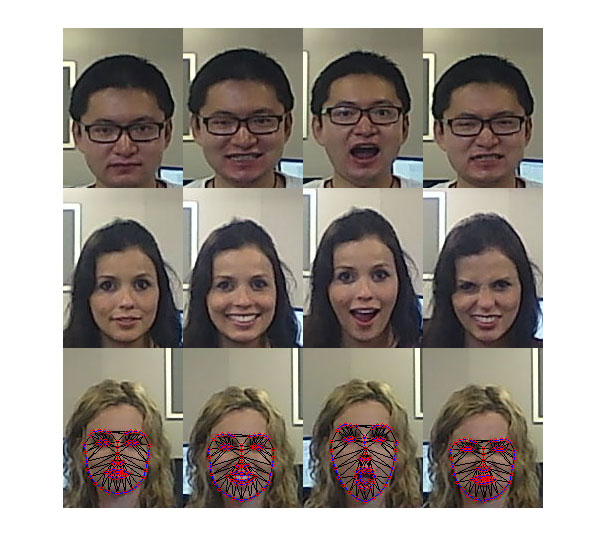
\includegraphics[width=0.95\textwidth,height=90mm]{figures/dataExtrationExamples.jpg}
\end{center}
\caption{\textbf{Data Gathering}. Fifty subjects overall were recruited  and asked to perform 11 types of facial shapes during a recording session.
We strove to  get a diverse representation of gender, ethnicity and age. The bottom row shows the facial tracker model superimpose 
over one of the subjects participating in the experiment.}
\label{comparationBetweenFaces}
\end{figure}

Each participant was given a chance to familiarize with the system and to try out  all the different facial expressions
to pose  during the data capture phase. After this familiarization process with the system the subject was told to
perform again the 11 face shapes. For every face shape recorded, 20 samples were recorded with a small time interval
between them (less than one second). Each sample consists on recording the invariant vector that transforms a neutral
face shape into the deformed face shape that fits the subject facial expression. Since there was fluctuations on the
borders of the face shape tracker and this generated some instability on the invariant vector, 20 samples to smooth out
this error. This data was subsequently used for training and validation.


During the data extraction period, we observed that every person had a unique invariant vector signature which was
specific for each facial expression on for different persons. We thought that this invariant feature vector could be
used to recognize people as well as facial expressions. The invariant feature vector specific for each person and
facial expression can be seen in the Figure \ref{comparationBetweenFaces}.

For the task of facial expression recognition, even though every person has its own unique feature vector signature for
each face expression, there is a similarity between these vectors when comparing the same face shape of different
people, thus the goal of the SVM was to generate an abstraction of each facial expression class in order to be able to
carry out facial expression classification.

\subsubsection{Data training}
The first experiment tried to recognize people's identity using the entire data set of the study participants. Three
different training conditions were used for this experiment. 10-fold cross validation was applied for all the conditions
during the validation procedure. The 3 training conditions analyzed were:

\begin{description}
\item[$\bullet$ Method 1:] Only the neutral face shape was used in this
experiment.  The training and test set data were generated by splitting 70\% of
the samples of each person to train and the remaining to test. The experiment was conducted by increasing the number 
of people in the experiment and testing the resulting accuracy.
\item[$\bullet$ Method 2:]Six face shapes were used in this experiment (neutral,
opened mouth, smiling, raised eyebrow, surprise and anger face). All of those
shapes were transformed into a unique class that corresponds to each
participant. The training and test set data were generated by splitting 70\% of
the samples of each person to train and the remaining to test. The procedure is conducted by
increasing the number of people in the experiment and testing the resulting
accuracy.
\item[$\bullet$ Method 3:]All the face shapes were used in this experiment. All
face shapes collected of one person were transformed into a unique class. The
training and test set data were generated by splitting 70\% of the samples of
each face shape to train and the remaining to test. The procedure is conducted
by increasing the number of people in the experiment and testing the resulting
accuracy.
\end{description}

For face shape recognition, there were three different methods of training that
were used throughout the experiments. All of them used a 7:3 ratio for testing 
and training set respectively. 10-fold cross validation was applied in all
methods during the validation procedure.

\begin{description}
\item[$\bullet$ Method 4:] All facial expression were used in this experiment.
The training and test set share the same group of participants but using
different  versions (captured in a different time slot) of the same face shape
for training and testing. The ratio is kept by assigning 70\% of the face shapes
of each person to the train set and 30\% to the test set. The procedure is conducted
by increasing the number of people in the experiment and testing the resulting
accuracy.
\item[$\bullet$ Method 5:] All facial expressions were used in this experiment,
the training and test set do not  share the same group of participants, the
ratio is kept by assigning 70\% of the people on the training set and 30\% on the
test set. The procedure is conducted by increasing the number of people in the
experiment and testing the results accuracy.
\item[$\bullet$ Method 6:] The sixth method had a different methodology, it was
used by all the participants but its goal was to analyze the impact on accuracy
on increasing the number of face shapes (classes).  The training and test set do
not share the same group of people, and the ratio was to assign 70\% of the whole set to
train and 30\% to test. The procedure is conducted by increasing the number of
face shapes (classes) in the experiment and testing the results accuracy.
\end{description}

\begin{figure}[ht]
\begin{center}
\vspace{-3mm}
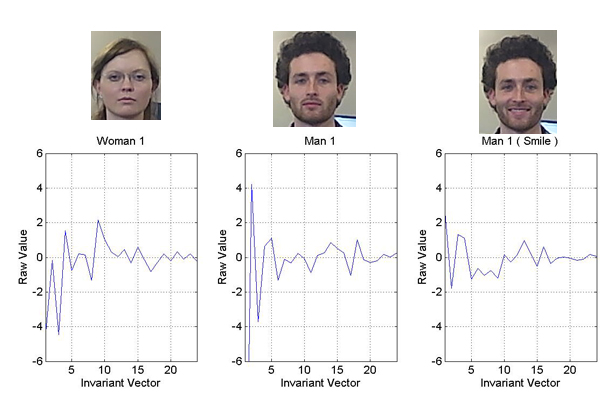
\includegraphics[width=0.95\textwidth,height=75mm]{figures/comparationBetweenFaces2.jpg}
\end{center}
\caption{\textbf{Invariant and Unique Feature Vectors of Facial Expressions.} this figure displays a. Typical feature 
vector signature specific for a given person. These constraint can be used to recognize people. The feature vector
provided by the face tracker changes for each facial expression perform but remains invariant we seen a given facial 
expression. Furthermore, features vectors of the same facial expression among different people share commonalities that
can be exploited to carry out facial expression recognition among different people.}
\label{comparationBetweenFaces}
\end{figure}s

\section{Results}

\subsection{Recognizing Facial Identity}
We tested first the ability of our classification algorithms to detect facial identity. In these set of experiments,
each person to be recognized represents a class. Therefore, increasing the number of people in the data set to recognize
increases the number of the classes, on the difficulty for the classification algorithm. We tested the performance of
the algorithm on the range of 2 to 50 people and under three different scenarios. These scenarios are described by
Method 1, Method 2 and Method 3, and can be summarized as representing data sets using only neutral face, 6 face shapes
and 11 face shapes.


It is expected that as we increase the number of people in the experiment, accuracy would be reduced due the growth of
classes of the problem. It is also expected  that using less face shapes to model one person reduces the complexity of
each class and thus this results in higher accuracy performance. Figure \ref{feRecognition}, shows that to recognize 50
people using only Neutral faces resulted in 98.1\% recognition accuracy.  Using 6 face shapes, accuracy decreases to
82.9\% and using 11 face shapes accuracy decreases further to 76.02\%.


\begin{figure}[ht]
\begin{center}
\vspace{-3mm}
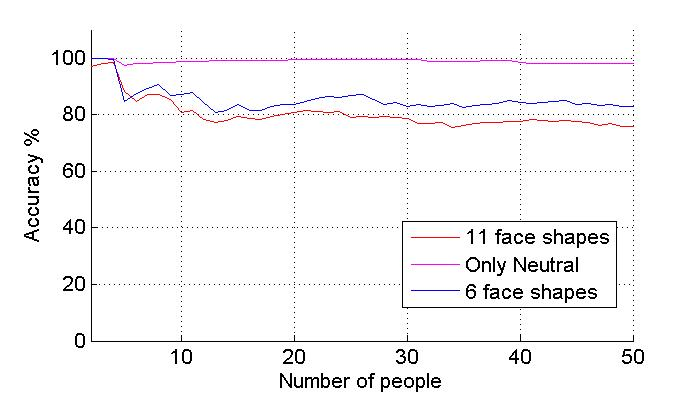
\includegraphics[width=0.95\textwidth]{figures/peopleRecognition4.jpg}
\end{center}
\caption{\textbf{Facial Identity Recognition Results.} the facial tracker engine used in this work can also be employed 
to recognize the identity of the face since the feature vector generated is very representative  of each different face.
Facial identity recognition performed very well when using the training set consisting of exclusively neutral faces. 
Performance degraded slightly as we increased the number of facial shapes in the training set, but still the system shows 
robust  recognition.}
\label{feRecognition}
\end{figure}



\subsection{Recognizing Face Expressions}
In this experiment, the goal was to recognize each of the 11 different classes of facial expressions in the training
set. We used all the 24 features of each face shape. We tested two different approaches on the results measurement.
These different approaches are described by the Method 4 and Method 5 in the Data training section.
For the first method (Method 4), since the group of people used in the training set is the same as that used on the test
set, and even though the data used in the test set was different compared to the training set, it was expected to have
high accuracy results. Note that since there was a separation from the training and test set population, the test set is
only 30\% of the total population (i.e. 50 people problem generate 15 people to the test set).
For the second method (Method 5), it was expected that as long as it is increased the number of people in the data, the
accuracy gradually would increase. As we can see on the Figure \ref{identityRecognition}, the accuracy obtained with 50 participants using the Method
4(Excluding) was 57.18\%, and using the Method 5(Including) was 97.5\%.
 

\begin{figure}[ht]
\begin{center}
\vspace{-3mm}
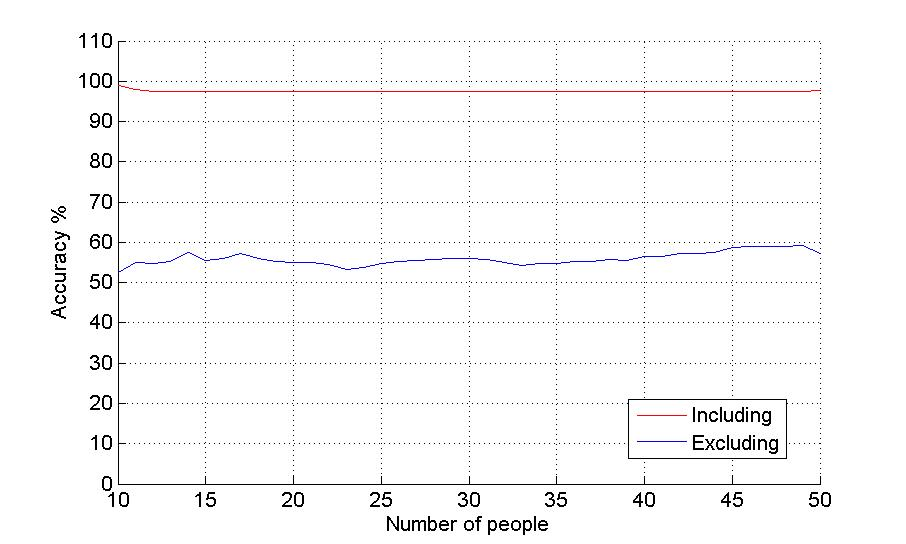
\includegraphics[width=0.95\textwidth]{figures/figureRecognizeFacialExpressionTrue.jpg}
\end{center}
\caption{\textbf{Facial Expression Recognition Results.} This figure shows the result of the facial expression recognition results.
The curve labeled ``including'' petition the data set to training and test sets, but that training and test sets belong to the same participants.
The curve labeled ``excluding'' represents the much harder problem of recognizing facial expressions of unknown subjects. Still, 
the performance of the system was quite robust as the number of people increased.}
\label{identityRecognition}
\end{figure}

 
\subsection{Recognizing Face Expressions results by changing the number of
classes}

Figure \ref{feRecognition} shows the results of increasing the number of people to be recognized by the classifier. In
this experiment, the goal was to evaluate the impact on accuracy of increasing  the number of classes to be recognized.
The Method 6 was used on this task. It was expected that the algorithm would gradually decrease in accuracy efficiency
as we included more facial expressions (classes). The accuracy for 4 classes was 95.1\% and for 7 classes was 73.2\%.


\begin{figure}[ht]
\begin{center}
\vspace{-3mm}
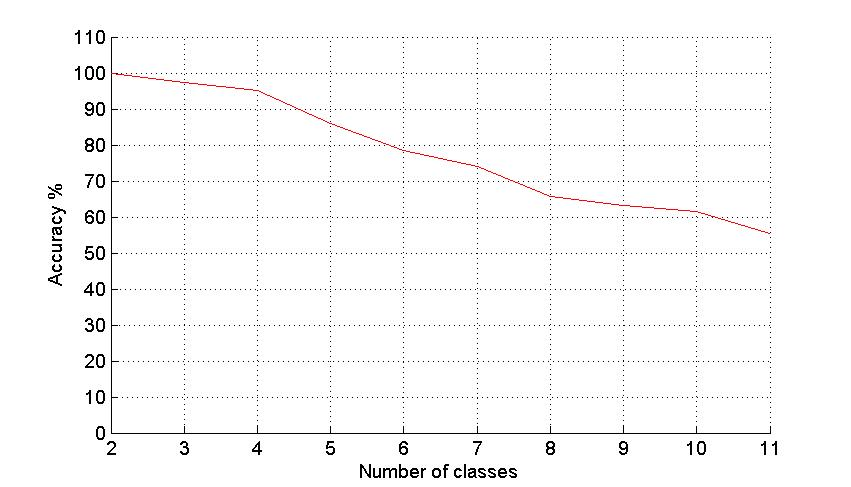
\includegraphics[width=0.95\textwidth]{figures/50people_increasing_classes.jpg}
\end{center}
\caption{\textbf{Effect of Increasing the Number of Facial Expressions to Recognize.} This figure displays how the 
performance of the system degrades as the number of classes or face shapes to recognize is increased. }
\label{increasingNumberExpressions}
\end{figure}


\section{Discussion}
In this work we have used an open-source face tracker based on regularised landmark mean-shift to recognize facial
identity and to classify facial expressions. The face tracker provided a feature vector invariant to scale, rotation and
translation transformations. A person adopting a given facial shape would generate on the face tracker an invariant
feature vector that we called through the paper signature vector. This signature vector would change with each facial
expression  and among different subjects. Still, the similarities among people adopting the same facial expression 
allowed for facial expression recognition of subjects unexposed to the system during training.


The proposed system shows an extremely strong performance for recognizing facial expressions of persons whose facial
expressions were used to train the system ( close to 100\%). performance degrades considerably when using the system to
recognize facial expressions of subjects that were not Jews during the training phase. Still, this is an extremely
challenging problem, and the performance of the system is encouraging and robust and not degrading even for relatively
large numbers of people.


Obviously the larger the amount of classes (facial expressions) to classify, the more challenging the
classification problem is. In this work, we did not limit ourselves to the traditional set  of six facial expressions
used in the literature on the subject. We've included additional facial expressions or more appropriately facial shapes
in order to test the performance of our approach in extreme environments. Obviously, the performance of the proposed
method degrades as the number of classes  on facial shapes increases, but these decrees is smooth with no abrupt
negative slopes as the number of facial shapes is increased over the different experimental trials.


When we observed the distinctive feature vectors signature associated to each individual face, we immediately thought
about the application of using the face tracker engine to recognize facial identity. The algorithm performed extremely
well  through the whole range of testing conditions that we tested ( using interfaces neutral faces, using six facial
shapes and using 11 facial shapes). The algorithm proved to be extremely robust to recognize the identity of face using
just an neutral face, with performance  almost as high as 100\%.

The initial motivation for this work was to test a face tracker in the recognition of facial expressions  to augment
existing gaze tracking systems enough to to provide additional information about the internal cognitive state of the
subject interfacing a computer system. We have shown that the data provided by these open-source face tracker is enough
on its own to generate a rich source of information that can be used to monitor a user. The open source nature of the
software makes its distribution and adoption by the research community extremely easy. Also, the very basic hardware
requirements required by the face tracker, just a normal web camera, further facilitates its adoption and dispersion
within the research community. 


In summary, we have shown here how an open source face tracker using regularized landmark main shift can be successfully
used to recognize facial identity and facial expression. Future work should try to integrate the data provided by the
eye tracker with the data provided by the face tracker in order to show how the combination of both tracking modalities
augments and improves the monitoring capabilities of either system on its own.





\bibliographystyle{plain}
\bibliography{library,extrabib}

\end{document}
